\section{The FRM Dataset}
In this section, we describe the detailed procedure of constructing \emph{Few-shot Relation-classification Medical} (FRM) dataset and show the dataset statistics. The whole procedure consists of three steps (Figure \ref{fig:construct}): (1) We crawl data from Chinese health-related websites to form a large corpus and an entity dictionary. (2) We automatically align the entities in the corpus with the entity dictionary, forming a large candidate-sentence set. (3) We manually filter out the unqualified candidate sentences and tag qualified ones with corresponding relation labels. Finally, we get a clean Chinese few-shot relation classification dataset in medical domain.

\begin{figure}
    \centering
    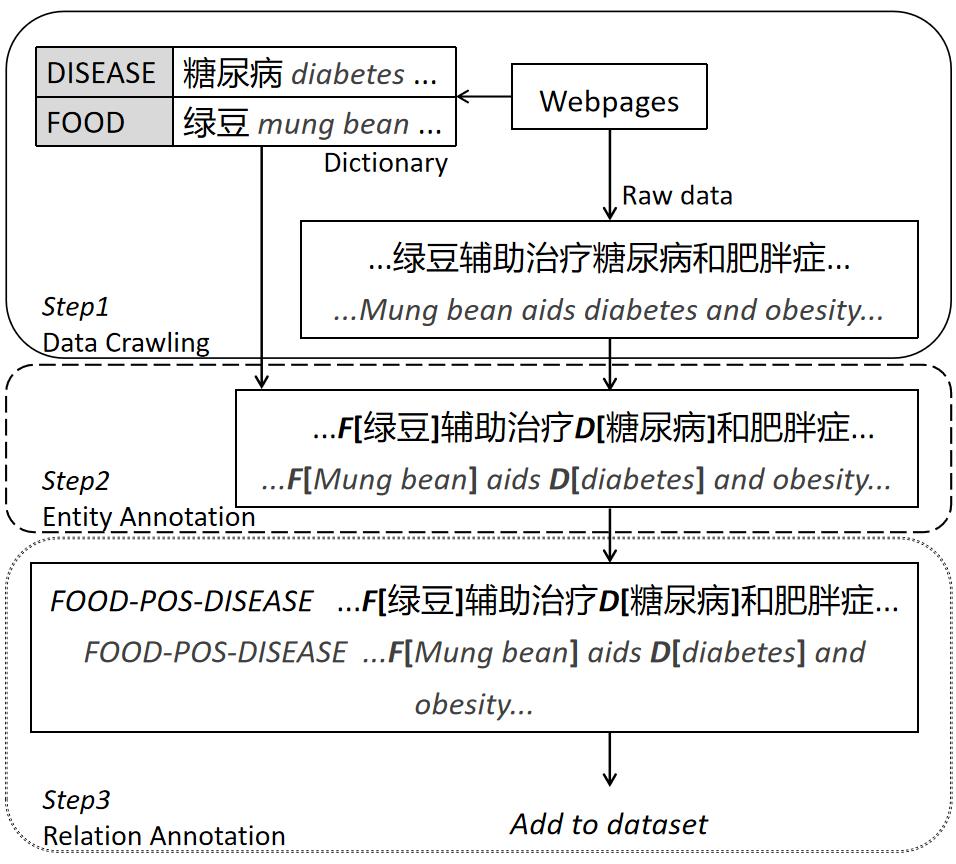
\includegraphics[width=8cm]{datasetconstruct.png}
    \caption{The construction procedure of FRM dataset.}
    \label{fig:construct}
\end{figure}

\subsection{Crawling Corpus and Entity Dictionaries}
The first step of constructing the FRM dataset is to obtain a Chinese medical corpus of considerable size and a dictionary containing different types of entities. Both the corpus and the dictionary is acquired by crawling Chinese health-related websites (\url{http://www.xywy.com},  \url{http://www.39.net} and \url{https://www.9939.com}). An example sentence from the crawled corpus and example entities from dictionaries are shown in Figure \ref{fig:construct} enclosed by the solid rectangle.
\subsection{Auto-labeling Entities}
We automatically align the entities in the dictionary to the sentences in corpus.

We firstly apply longest-exact match to extract sentences that contain two entities in the dictionary. In the longest-exact match procedure, for a candidate string $s$, we denote a substring of length $l$ starting from the $i^{th}$ character as $s_{i,l}$. We adopt a boolean function $m$ where $m(s_{i,l})=True$ if substring $s_{i,l}$ exactly matches an entity in the dictionary, and $False$ otherwise. We go through $s$ from left to right. If $m(s_{i,l})=True$ and there is no $s_{j,k}$ that satisfies (1) $s_{j,k}$ contains $s_{i,l}$ (2)$m(s_{i,l})=True$, we call $s_{i,l}$ a longest matched substring. If a sentence contains two distinct longest matched substrings, we label these two substrings as entities $e$ and add this sentence to a set of candidate sentences.

Then, for each candidate sentence $s$ with entities $e$ labeled, we perform word segmentation on $s$ to split it into words $\{w_0,w_1,...,w_t\}$ where $t$ is the length of the sentence. We assert that for either entity $e_i,i=0,1$ in $e$, it must satisfies $e_i=join(w_j,...w_k)$ for $\forall j,k \in [0...t-1]$ where $join$ is a string joining function. If the requirement is not met, we discard this sentence. Thus only sentences with $e$ that are compete words remain. Example is shown in Figure \ref{fig:construct} the dashed rectangle.
\subsection{Manual Screening and Relation-labeling}
We manually screen out the remaining entity-wrongly-labeled candidate sentences. For each correctly-labeled sentence $s$, we manually tag the relation $r$ to the sentence. Thus we get a triple $(s,e,r)$ and add the triple into the dataset. Example is shown in the dotted rectangle in Figure \ref{fig:construct}.
Relations are manually annotated because of the noise in the crawled sources and the semantic ambiguity issues.
\subsection{Dataset Statistics}


\begin{table}[ht]
\centering
\small
\begin{tabu}{|c|[0.5pt]l|}
\hline
\textbf{Group} & \textbf{Relations} \\ \tabucline[0.5pt]{-}
D-D & complication, cause, is, include, NA \\ \hline
D-S & have, NA\\ \hline
D-F & positive, negative, forbid, prevent, cause, NA\\ \hline
D-N & positive, negative, prevent, lack, cause, NA\\ \hline
F-N & contain, NA\\ \hline
S-F & forbid, cause, positive, negative, prevent, NA\\ \hline
\end{tabu}
\caption{Entity groups in FRM dataset. D,S,F,N stands for Disease, Symptom, Food and Nutrient respectively.}
\label{Egroup}
\end{table}

The FRM dataset contains 27 relations with 50 instances per relation. The 27 relations cover binary relations among 4 entity types. The average length of a sentence in FRM dataset is 67.62, and there are totally 2,187 unique characters.

The 27 relations in FRM dataset can be aggregated into 6 groups according to the entity types (Table \ref{Egroup}). We use separated relations for training and testing. More meaningfully, when treating one group of relations as the test set, other groups serve as the training set. Thus, we can formulate 6 different few-shot relation classification tasks with our FRM dataset.

\begin{table}[ht]
\centering
\small
\begin{tabular}{|l|r|r|r|}
\hline
\textbf{Dataset} & \textbf{\#cls.} & \textbf{\#inst./cls.} & \textbf{\#inst.} \\ \hline
FewRel & 100 & 700 & 70,000 \\ \hline
FRM & 27 & 50 & 1,350 \\ \hline
\end{tabular}
\caption{Comparison of FRM dataset to other few-shot relation classification datasets.}
\label{Datasetcompare}
\end{table}


The FRM dataset provides hard tasks for several reasons. Firstly, we shrink the training data size. Table \ref{Datasetcompare} shows the comparison of data size with previous few-shot relation classification datasets. Secondly, the relations in a given test set are relative to each other since the share common entity types (because the relations are from the same group). In other datasets, the entity types are distinct in most situations, which may serve as extra information. %Figure xx shows example instances from previous datasets and the HEALTHXX dataset. For previous datasets, the instances within the same category is likely to be quite similar while instances from different categories distinct from one to another. While in HEALTHXX datasets, the format of instances within one category varies from one to another, which makes the task harder.

The detailed meaning and example instances of each relation is listed in Appendix ...
